\batchmode
\makeatletter
\def\input@path{{/Users/sergei.winitzki/Code/talks/ftt-fp/}}
\makeatother
\documentclass[english]{beamer}
\usepackage[T1]{fontenc}
\usepackage[latin9]{inputenc}
\setcounter{secnumdepth}{3}
\setcounter{tocdepth}{3}
\usepackage{babel}
\usepackage{amsmath}
\usepackage{graphicx}
\ifx\hypersetup\undefined
  \AtBeginDocument{%
    \hypersetup{unicode=true,pdfusetitle,
 bookmarks=true,bookmarksnumbered=false,bookmarksopen=false,
 breaklinks=false,pdfborder={0 0 1},backref=false,colorlinks=true}
  }
\else
  \hypersetup{unicode=true,pdfusetitle,
 bookmarks=true,bookmarksnumbered=false,bookmarksopen=false,
 breaklinks=false,pdfborder={0 0 1},backref=false,colorlinks=true}
\fi

\makeatletter

%%%%%%%%%%%%%%%%%%%%%%%%%%%%%% LyX specific LaTeX commands.
%% Because html converters don't know tabularnewline
\providecommand{\tabularnewline}{\\}

%%%%%%%%%%%%%%%%%%%%%%%%%%%%%% Textclass specific LaTeX commands.
 % this default might be overridden by plain title style
 \newcommand\makebeamertitle{\frame{\maketitle}}%
 % (ERT) argument for the TOC
 \AtBeginDocument{%
   \let\origtableofcontents=\tableofcontents
   \def\tableofcontents{\@ifnextchar[{\origtableofcontents}{\gobbletableofcontents}}
   \def\gobbletableofcontents#1{\origtableofcontents}
 }
 \newenvironment{lyxcode}
   {\par\begin{list}{}{
     \setlength{\rightmargin}{\leftmargin}
     \setlength{\listparindent}{0pt}% needed for AMS classes
     \raggedright
     \setlength{\itemsep}{0pt}
     \setlength{\parsep}{0pt}
     \normalfont\ttfamily}%
    \def\{{\char`\{}
    \def\}{\char`\}}
    \def\textasciitilde{\char`\~}
    \item[]}
   {\end{list}}

%%%%%%%%%%%%%%%%%%%%%%%%%%%%%% User specified LaTeX commands.
\usetheme[secheader]{Boadilla}
\usecolortheme{seahorse}
\title[Generating code with Curry-Howard]{Generating code from type signatures
using the Curry-Howard correspondence}
\subtitle{With implementations in Haskell and Scala}
\author{Sergei Winitzki}
\date{March 22, 2018}
\institute[BAHUG]{Bay Area Haskell Users' Group}
\setbeamertemplate{headline}{} % disable headline at top
\setbeamertemplate{navigation symbols}{}

\makeatother

\begin{document}
\frame{\titlepage}
\begin{frame}{Type-directed coding}

How to implement functions given their type?

We write code ``guided by the types''
\begin{enumerate}
\item Implement \texttt{\textcolor{blue}{\footnotesize{}fmap}} for the Reader
monad,{\footnotesize{}
\[
\text{fmap}::\left(a\rightarrow b\right)\rightarrow\left(e\rightarrow a\right)\rightarrow\left(e\rightarrow b\right)
\]
}{\footnotesize \par}
\item Show that one cannot implement{\footnotesize{} $\left(e\rightarrow f\right)\rightarrow\left(e\rightarrow a\right)\rightarrow\left(f\rightarrow a\right)$}{\footnotesize \par}
\item Implement {\footnotesize{}$\text{fmap}::\left(a\rightarrow b\right)\rightarrow\left(e\rightarrow\text{Maybe}\,a\right)\rightarrow\left(e\rightarrow\text{Maybe}\,b\right)$}{\footnotesize \par}
\item Implement the distributive law: \texttt{\textcolor{blue}{\footnotesize{}
\[
\left(A+B\right)\times C\Leftrightarrow A\times C+B\times C
\]
}}{\footnotesize \par}
\end{enumerate}
Often, there is only one ``useful'' implementation

The \texttt{\textcolor{blue}{\footnotesize{}djinn}} and \texttt{\textcolor{blue}{\footnotesize{}curryhoward}}
libraries try to generate that implementation
\begin{itemize}
\item The \href{https://hackage.haskell.org/package/djinn-ghc}{djinn-ghc}
compiler plugin and the \href{https://github.com/nomeata/ghc-justdoit}{JustDoIt plugin}
generate Haskell code from type (need \href{https://github.com/serras/emacs-haskell-tutorial/blob/master/tutorial.md\#working-with-holes}{tooling}
to use)
\item The \href{https://github.com/Chymyst/curryhoward}{curryhoward} library
generates Scala code from type 
\end{itemize}
\end{frame}

\begin{frame}{Haskell: Using the \texttt{djinn} tool}


\framesubtitle{Demo time}

Features:
\begin{itemize}
\item Haskell syntax, supports algebraic data types and type classes
\item Constant types (\texttt{\textcolor{blue}{\footnotesize{}Int}}, \texttt{\textcolor{blue}{\footnotesize{}String}},
etc.) are treated as type parameters
\item If several implementations are available, chooses ``intelligently''
\item Can output several implementations if desired
\end{itemize}
Examples:
\begin{lyxcode}
\textcolor{blue}{\footnotesize{}Djinn>~f1~?~(a~->~b)~->~(e~->~a)~->~(e~->~b)}{\footnotesize \par}

\textcolor{blue}{\footnotesize{}f1~::~(a~->~b)~->~(e~->~a)~->~e~->~b}{\footnotesize \par}

\textcolor{blue}{\footnotesize{}f1~a~b~c~=~a~(b~c)}{\footnotesize \par}

\textcolor{blue}{\footnotesize{}Djinn>~f2~?~(a,~a,~a)~->~Maybe~(a,~a,~a)~}{\footnotesize \par}

\textcolor{blue}{\footnotesize{}f~::~(a,~a,~a)~->~Maybe~(a,~a,~a)}{\footnotesize \par}

\textcolor{blue}{\footnotesize{}f~(a,~b,~c)~=~Just~(c,~b,~a)}{\footnotesize \par}
\end{lyxcode}
\end{frame}

\begin{frame}{Scala: Using the \texttt{curryhoward} library}

Two main use cases:
\begin{enumerate}
\item Define a method and provide an automatic implementation
\begin{lyxcode}
\textcolor{blue}{\footnotesize{}def~map{[}E,~A,~B{]}(readerA:~E~$\Rightarrow$~A,~f:~A~$\Rightarrow$~B):~E~$\Rightarrow$~B~=~implement}{\footnotesize \par}
\end{lyxcode}
\item Automatically build an expression from previously computed values
\begin{lyxcode}
\textcolor{blue}{\footnotesize{}val~f:~String~$\Rightarrow$~Boolean~$\Rightarrow$~Int~=~\{...\}}{\footnotesize \par}

\textcolor{blue}{\footnotesize{}case~class~Result(x:~Int,~name:~String)}{\footnotesize \par}

\textcolor{blue}{\footnotesize{}val~result~=~ofType{[}Result{]}(\textquotedbl{}abc\textquotedbl{},~f,~true)}{\footnotesize \par}
\end{lyxcode}
\end{enumerate}
Features:
\begin{itemize}
\item Compile-time code generation via Scala macros
\item Supports functions, tuples, sealed trait / case classes / case objects
\item Constant types (\texttt{\textcolor{blue}{\footnotesize{}Int}}, \texttt{\textcolor{blue}{\footnotesize{}String}},
etc.) are treated as type parameters
\item If several implementations are available, chooses ``intelligently''
\item Lambda-calculus evaluator available for symbolic law checking
\end{itemize}
\end{frame}

\begin{frame}{Benefits and limitations of this method}

Benefits:
\begin{itemize}
\item Save time implementing ``trivial'' functions
\item With some more work, can verify algebraic laws
\item In many practical use cases, supports type class derivation
\end{itemize}
Limitations:
\begin{itemize}
\item Heuristics often fail with certain kinds of data (repeated types)
\item Cannot generate recursive code
\item Cannot depend on existing type class instances (\texttt{\textcolor{blue}{\footnotesize{}Functor
f $\Rightarrow$ ...}})
\end{itemize}
\end{frame}

\begin{frame}{Type constructions in functional programming}


\framesubtitle{The common ground between Haskell, Scala, Rust, OCaml, and other
languages}

Type constructions common in FP languages:
\begin{itemize}
\item Tuple (``product'') type: $\text{Int}\times\text{String}$
\item Function type: $\text{Int}\Rightarrow\text{String}$
\item Disjunction (``sum'') type: $\text{Int}+\text{String}$
\item Unit type (``empty tuple''): $1$
\item Type parameters: $\text{List}^{T}$
\end{itemize}
Up to differences in syntax, the FP languages share all these features
\end{frame}

\begin{frame}{Type constructions: Haskell syntax}

\begin{itemize}
\item Tuple type: \texttt{\textcolor{blue}{\footnotesize{}(Int, String)}}{\footnotesize \par}
\begin{itemize}
\item Create: \texttt{\textcolor{blue}{\footnotesize{}pair = (123, \textquotedbl{}abc\textquotedbl{})}} 
\item Use: \texttt{\textcolor{blue}{\footnotesize{}(\_, y) = pair}}{\footnotesize \par}
\end{itemize}
\item Function type: \texttt{\textcolor{blue}{\footnotesize{}Int -> String}}{\footnotesize \par}
\begin{itemize}
\item Create: \texttt{\textcolor{blue}{\footnotesize{}f = \textbackslash{}x
-> \textquotedbl{}Value is \textquotedbl{} ++ show x}} 
\item Use: \texttt{\textcolor{blue}{\footnotesize{}y = f 123}}{\footnotesize \par}
\end{itemize}
\item Disjunction type: \texttt{\textcolor{blue}{\footnotesize{}data E =
Left Int | Right String}}{\footnotesize \par}
\begin{itemize}
\item Create:\\
\  \texttt{\textcolor{blue}{\footnotesize{}x = Left 123}}~\\
\texttt{\textcolor{blue}{\footnotesize{} y = Right \textquotedbl{}abc\textquotedbl{}}}{\footnotesize \par}
\item Use: \texttt{\textcolor{blue}{\footnotesize{}z = case x of}}~\\
\texttt{\textcolor{blue}{\footnotesize{} Left i -> i > 0}}~\\
\texttt{\textcolor{blue}{\footnotesize{} Right \_ -> false}}~\\
{\footnotesize \par}
\end{itemize}
\item Unit type: \texttt{\textcolor{blue}{\footnotesize{}Unit}}{\footnotesize \par}
\begin{itemize}
\item Create: \texttt{\textcolor{blue}{\footnotesize{}x = ()}}{\footnotesize \par}
\end{itemize}
\end{itemize}
\end{frame}

\begin{frame}{Type constructions: Scala syntax}

\begin{itemize}
\item Tuple type: \texttt{\textcolor{blue}{\footnotesize{}(Int, String)}}{\footnotesize \par}
\begin{itemize}
\item Create: \texttt{\textcolor{blue}{\footnotesize{}val pair:\ (Int,
String) = (123, \textquotedbl{}abc\textquotedbl{})}} 
\item Use: \texttt{\textcolor{blue}{\footnotesize{}val y:\ String = pair.\_2}}{\footnotesize \par}
\end{itemize}
\item Function type: \texttt{\textcolor{blue}{\footnotesize{}Int $\Rightarrow$
String}}{\footnotesize \par}
\begin{itemize}
\item Create: \texttt{\textcolor{blue}{\footnotesize{}def f:\ (Int $\Rightarrow$
String) = x $\Rightarrow$ \textquotedbl{}Value is \textquotedbl{}
+ x.toString}} 
\item Use: \texttt{\textcolor{blue}{\footnotesize{}val y:\ String = f(123)}}{\footnotesize \par}
\end{itemize}
\item Disjunction type: \texttt{\textcolor{blue}{\footnotesize{}Either{[}Int,
String{]}}} defined in standard library
\begin{itemize}
\item Create:\\
 \texttt{\textcolor{blue}{\footnotesize{}\ val x:\ Either{[}Int,
String{]} = Left(123)}}~\\
\texttt{\textcolor{blue}{\footnotesize{} val y:\ Either{[}Int, String{]}
= Right(\textquotedbl{}abc\textquotedbl{})}}{\footnotesize \par}
\item Use: \texttt{\textcolor{blue}{\footnotesize{}val z:\ Boolean = x
match \{}}~\\
\texttt{\textcolor{blue}{\footnotesize{} case Left(i) $\Rightarrow$
i > 0}}~\\
\texttt{\textcolor{blue}{\footnotesize{} case Right(\_) $\Rightarrow$
false}}~\\
\texttt{\textcolor{blue}{\footnotesize{}\}}}{\footnotesize \par}
\end{itemize}
\item Unit type: \texttt{\textcolor{blue}{\footnotesize{}Unit}}{\footnotesize \par}
\begin{itemize}
\item Create: \texttt{\textcolor{blue}{\footnotesize{}val x:\ Unit = ()}}{\footnotesize \par}
\end{itemize}
\end{itemize}
\end{frame}

\begin{frame}{From types to propositions}

The code \texttt{\textcolor{blue}{\footnotesize{}x::\ t; x =}} ...
shows that \emph{we can compute a value} of type \texttt{\textcolor{blue}{\footnotesize{}t}}
as part of our program expression
\begin{itemize}
\item Let's denote this \emph{proposition} by ${\cal CH}(t)$ \textendash{}
``$\mathcal{C}$ode $\mathcal{H}$as a value of type \texttt{\textcolor{blue}{\footnotesize{}t}}''
\item Correspondence between types and propositions, for a given program:
\end{itemize}
\begin{center}
\begin{tabular}{|c|c|c|}
\hline 
\textbf{Type} &
\textbf{Proposition} &
\textbf{Short notation}\tabularnewline
\hline 
\hline 
\texttt{\textcolor{blue}{\footnotesize{}t}} &
${\cal CH}(t)$ &
$t$\tabularnewline
\hline 
\texttt{\textcolor{blue}{\footnotesize{}(a, b)}} &
${\cal CH}(a)$ \emph{and} ${\cal CH}(b)$ &
$a\wedge b$; $a\times b$\tabularnewline
\hline 
\texttt{\textcolor{blue}{\footnotesize{}A a | B b}} &
${\cal CH}(a)$ \emph{or} ${\cal CH}(b)$ &
$a\vee b$; $a+b$\tabularnewline
\hline 
\texttt{\textcolor{blue}{\footnotesize{}a $\rightarrow$ b}} &
${\cal CH}(a)$ \emph{implies} ${\cal CH}(b)$ &
$a\Rightarrow b$\tabularnewline
\hline 
\texttt{\textcolor{blue}{\footnotesize{}()}} &
\emph{True} &
1\tabularnewline
\hline 
\end{tabular}
\par\end{center}
\begin{itemize}
\item Type parameter in a function type means $\forall t$
\item Example: \texttt{\textcolor{blue}{\footnotesize{}dupl::\ a $\rightarrow$
(a, a)}}. The type of this function, $a\Rightarrow a\times a$, corresponds
to the theorem $\forall a:a\Rightarrow a\wedge a$
\end{itemize}
\end{frame}

\begin{frame}{Translating language constructions into the logic I}


\framesubtitle{How to represent logical relationships between ${\cal CH}(...)$
propositions?}

Code expressions create\,\emph{logical relationships} between propositions
${\cal CH}(...)$
\begin{itemize}
\item ``Logical relationships'' = what will be true if something given
is true
\item The elementary proof task is represented by a \textbf{sequent}
\begin{itemize}
\item Notation: $A,B,C\vdash G$; the \textbf{premises} are $A,B,C$ and
the \textbf{goal} is G
\end{itemize}
\item Proofs are achieved via axioms and derivation rules
\begin{itemize}
\item Axioms: such and such sequents are already true
\item Derivation rules: this sequent is true if such and such sequents are
true
\end{itemize}
\item To make connection with logic, represent code fragments as \textbf{sequents}
\item \textcolor{blue}{$a,b\vdash c$} represents an \emph{expression} of
type \texttt{\textcolor{blue}{\footnotesize{}c}} that uses \texttt{\textcolor{blue}{\footnotesize{}x
::\ a}} and \texttt{\textcolor{blue}{\footnotesize{}y ::\ b}}{\footnotesize \par}
\item Examples in Haskell (assume \texttt{\textcolor{blue}{\footnotesize{}x
::\ Int}}):
\begin{itemize}
\item \texttt{\textcolor{blue}{\footnotesize{}show x ++ \textquotedbl{}abc\textquotedbl{}}}
is an expression of type \texttt{\textcolor{blue}{\footnotesize{}String}}
that uses an \texttt{\textcolor{blue}{\footnotesize{}x::\ Int}},
and is represented by the sequent $\text{Int}\vdash\text{String}$
\item \texttt{\textcolor{blue}{\footnotesize{}\textbackslash{}x $\rightarrow$
show x + \textquotedbl{}abc\textquotedbl{}}} is an expression of type
\texttt{\textcolor{blue}{\footnotesize{}Int $\rightarrow$ String}}
and is represented by the sequent $\emptyset\vdash\text{Int}\Rightarrow\text{String}$
\end{itemize}
\item Sequents only describe the \emph{types} of expressions and their parts
\end{itemize}
\end{frame}

\begin{frame}{Translating language constructions into the logic II}


\framesubtitle{What are the derivation rules for the logic of types?}

Write all the constructions in FP languages as sequents
\begin{itemize}
\item This will give all the derivation rules for the logic of types
\begin{itemize}
\item Each type construction has an expression for creating it and an expression
for using it
\end{itemize}
\item Tuple type $A\times B$
\begin{itemize}
\item Create: $A,B\vdash A\times B$ 
\item Use: $A\times B\vdash A$ and also $A\times B\vdash B$
\end{itemize}
\item Function type $A\Rightarrow B$
\begin{itemize}
\item Create: if we have $A\vdash B$ then we will have $\emptyset\vdash A\Rightarrow B$ 
\item Use: $A\Rightarrow B,A\vdash B$
\end{itemize}
\item Disjunction type $A+B$
\begin{itemize}
\item Create: $A\vdash A+B$ and also $B\vdash A+B$
\item Use: $A+B,A\Rightarrow C,B\Rightarrow C\vdash C$
\end{itemize}
\item Unit type $1$
\begin{itemize}
\item Create: $\emptyset\vdash1$
\end{itemize}
\end{itemize}
\end{frame}

\begin{frame}{Translating language constructions into the logic III}


\framesubtitle{Additional rules for the logic of types}

In addition to constructions that use types, we have ``trivial''
constructions:
\begin{itemize}
\item a single, unmodified value of type $A$ is a valid expression of type
$A$
\begin{itemize}
\item For any $A$ we have the sequent $A\vdash A$
\end{itemize}
\item if a value can be computed using some given data, it can also be computed
if given\,\emph{additional} data
\begin{itemize}
\item If we have $A,...,C\vdash G$ then also $A,...,C,D\vdash G$ for any
$D$
\item For brevity, we denote by $\Gamma$ a sequence of arbitrary premises
\end{itemize}
\item the order in which data is given does not matter, we can still compute
all the same things given the same premises in different order
\begin{itemize}
\item If we have $\Gamma,A,B\vdash G$ then we also have $\Gamma,B,A\vdash G$
\end{itemize}
\end{itemize}
Syntax conventions:
\begin{itemize}
\item the implication operation associates \emph{to the right}
\begin{itemize}
\item $A\Rightarrow B\Rightarrow C$ means $A\Rightarrow\left(B\Rightarrow C\right)$
\end{itemize}
\item precedence order: implication, disjunction, conjunction
\begin{itemize}
\item $A+B\times C\Rightarrow D$ means $\left(A+\left(B\times C\right)\right)\Rightarrow D$
\end{itemize}
\end{itemize}
Quantifiers: implicitly, all our type variables are universally quantified
\begin{itemize}
\item When we write $A\Rightarrow B\Rightarrow A$, we mean $\forall A:\forall B:A\Rightarrow B\Rightarrow A$
\end{itemize}
\end{frame}

\begin{frame}{The logic of types I}

Now we have all the axioms and the derivation rules of the logic of
types.
\begin{itemize}
\item What theorems can we derive in this logic?
\item Example: $A\Rightarrow B\Rightarrow A$
\begin{itemize}
\item Start with an axiom $A\vdash A$; add an unused extra premise $B$:
$A,B\vdash A$
\item Use the ``create function'' rule with $B$ and $A$, get $A\vdash B\Rightarrow A$
\item Use the ``create function'' rule with $A$ and $B\Rightarrow A$,
get the final sequent $\emptyset\vdash A\Rightarrow B\Rightarrow A$
showing that $A\Rightarrow B\Rightarrow A$ is a \textbf{theorem}
since it is derived from no premises
\end{itemize}
\item What code does this describe?
\begin{itemize}
\item The axiom $A\vdash A$ represents the expression $x^{A}$ where $x$
is of type $A$
\item The unused premise $B$ corresponds to unused variable $y^{B}$ of
type $B$
\item The ``create function'' rule gives the function $y^{B}\Rightarrow x^{A}$
\item The second ``create function'' rule gives $x^{A}\Rightarrow\left(y^{B}\Rightarrow x\right)$
\item Haskell code:
\end{itemize}
\begin{lyxcode}
\textcolor{blue}{\footnotesize{}f~::~A~$\rightarrow$~B~$\rightarrow$~A}{\footnotesize \par}

\textcolor{blue}{\footnotesize{}f~=~\textbackslash{}x~$\rightarrow$~\textbackslash{}y~$\rightarrow$~x}{\footnotesize \par}
\end{lyxcode}
\item Any code expression's type can be translated into a sequent
\item A proof of a theorem directly guides us in writing code for that type
\end{itemize}
\end{frame}

\begin{frame}{Correspondence between programs and proofs}

\begin{itemize}
\item By construction, any theorem can be implemented in code
\end{itemize}
\begin{center}
\begin{tabular}{|c|c|}
\hline 
\textbf{Proposition} &
\textbf{Code}\tabularnewline
\hline 
\hline 
$\forall A:A\Rightarrow A$ &
\texttt{\textcolor{blue}{\footnotesize{}identity x = x}}\tabularnewline
\hline 
$\forall A:A\Rightarrow1$ &
\texttt{\textcolor{blue}{\footnotesize{}toUnit x = ()}}\tabularnewline
\hline 
$\forall A\forall B:A\Rightarrow A+B$ &
\texttt{\textcolor{blue}{\footnotesize{}Left :: a $\rightarrow$ Either
a b}}\tabularnewline
\hline 
$\forall A\forall B:A\times B\Rightarrow A$ &
\texttt{\textcolor{blue}{\footnotesize{}fst :: (a, b) $\rightarrow$
a}}\tabularnewline
\hline 
$\forall A\forall B:A\Rightarrow B\Rightarrow A$ &
\texttt{\textcolor{blue}{\footnotesize{}const = \textbackslash{}x
$\rightarrow$ \textbackslash{}y $\rightarrow$ x}}\tabularnewline
\hline 
\end{tabular}
\par\end{center}
\begin{itemize}
\item Also, non-theorems \emph{cannot be implemented} in code 
\begin{itemize}
\item Examples of non-theorems:\\
 $\forall A:1\Rightarrow A$; \  \  $\quad\forall A\forall B:A+B\Rightarrow A$;
\\
$\forall A\forall B:A\Rightarrow A\times B$; \  $\quad\forall A\forall B:(A\Rightarrow B)\Rightarrow A$
\end{itemize}
\item Given a type's formula, can we implement it in code? Not obvious.
\begin{itemize}
\item Example: $\forall A\forall B:((((A\Rightarrow B)\Rightarrow A)\Rightarrow A)\Rightarrow B)\Rightarrow B$
\begin{itemize}
\item Can we write a function with this type? Can we prove this formula?
\end{itemize}
\end{itemize}
\end{itemize}
\end{frame}

\begin{frame}{The logic of types II}


\framesubtitle{What kind of logic is this? What do mathematicians call this logic?}

This is called ``intuitionistic propositional logic'', IPL (also
``constructive'')
\begin{itemize}
\item This is a ``nonclassical'' logic because it is different from Boolean
logic
\item Disjunction works very differently from Boolean logic
\begin{itemize}
\item Example: $A\Rightarrow B+C\vdash(A\Rightarrow B)+(A\Rightarrow C)$
does not hold in IPL
\item This is counter-intuitive!
\item We cannot implement a function with this type:
\end{itemize}
\begin{lyxcode}
\textcolor{blue}{\footnotesize{}q~::~(a~$\rightarrow$~Either~b~c)~$\rightarrow$~Either~(a~$\rightarrow$~b)~(a~$\rightarrow$~c)}{\footnotesize \par}
\end{lyxcode}
\begin{itemize}
\item Disjunction is ``constructive'': need to supply one of the parts
\begin{itemize}
\item ...but \texttt{\textcolor{blue}{\footnotesize{}Either (a $\rightarrow$
b) (a $\rightarrow$ c)}} is not a function of \texttt{\textcolor{blue}{\footnotesize{}a}} 
\end{itemize}
\end{itemize}
\item Implication works somewhat differently
\begin{itemize}
\item Example: $\left(\left(A\Rightarrow B\right)\Rightarrow A\right)\Rightarrow A$
holds in Boolean logic but not in IPL
\item Cannot compute an \texttt{\textcolor{blue}{\footnotesize{}x ::\ A}}
because of insufficient data
\end{itemize}
\item Conjunction works the same as in Boolean logic
\begin{itemize}
\item Example: 
\[
A\Rightarrow B\times C\vdash\left(A\Rightarrow B\right)\times\left(A\Rightarrow C\right)
\]
 
\end{itemize}
\end{itemize}
\end{frame}

\begin{frame}{The logic of types III}


\framesubtitle{How to determine whether a given IPL formula is a theorem?}
\begin{itemize}
\item The IPL cannot have a truth table with a fixed number of truth values
\begin{itemize}
\item This was shown by G\"odel in 1932 (see \href{https://en.wikipedia.org/wiki/Many-valued_logic}{Wikipedia page})
\end{itemize}
\item The IPL has a decision procedure (algorithm) that either finds a proof
for a given IPL formula, or determines that there is no proof
\item There may be several inequivalent proofs of an IPL theorem
\item Each proof can be \emph{automatically translated} into code
\begin{itemize}
\item The \href{https://hackage.haskell.org/package/djinn-ghc}{djinn-ghc}
compiler plugin and the \href{https://github.com/nomeata/ghc-justdoit}{JustDoIt plugin}
implement an IPL prover in Haskell, and generate Haskell code from
types
\item The \href{https://github.com/Chymyst/curryhoward}{curryhoward} library
implements an IPL prover as a Scala macro, and generates Scala code
from types
\end{itemize}
\item All these IPL provers use the same basic algorithm called LJT 
\begin{itemize}
\item and all cite the same paper {\footnotesize{}\href{https://rd.host.cs.st-andrews.ac.uk/publications/jsl57.pdf}{[Dyckhoff 1992]}}{\footnotesize \par}
\item because most other papers on this subject are incomprehensible to
non-specialists, or describe algorithms that are too complicated
\end{itemize}
\end{itemize}
\end{frame}

\begin{frame}{Proof search I: looking for an algorithm}


\framesubtitle{Why our initial presentation of IPL does not give a proof search
algorithm}

The FP type constructions give nine axioms and three derivation rules:

\begin{minipage}[t]{0.49\columnwidth}%
\begin{itemize}
\item $\Gamma,A,B\vdash A\times B$ 
\item $\Gamma,A\times B\vdash A$ 
\item $\Gamma,A\times B\vdash B$
\item $\Gamma,A\Rightarrow B,A\vdash B$
\item $\Gamma,A\vdash A+B$ 
\item $\Gamma,B\vdash A+B$
\item $\Gamma,A+B,A\Rightarrow C,B\Rightarrow C\vdash C$
\item $\Gamma\vdash1$
\item $\Gamma,A\vdash A$
\end{itemize}
%
\end{minipage}%
\begin{minipage}[t]{0.49\columnwidth}%
\[
\frac{\Gamma,A\vdash B}{\Gamma\vdash A\Rightarrow B}
\]
\[
\frac{\Gamma\vdash G}{\Gamma,D\vdash G}
\]
\[
\frac{\Gamma,A,B\vdash G}{\Gamma,B,A\vdash G}
\]
%
\end{minipage}

\medskip{}
Can we use these rules to obtain a finite and complete search tree?
No.
\begin{itemize}
\item Try proving $A,B+C\vdash A\times B+C$: cannot find matching rules
\begin{itemize}
\item Need a better formulation of the logic
\end{itemize}
\end{itemize}
\end{frame}

\begin{frame}{Proof search II: Gentzen's calculus LJ (1935)}

\begin{itemize}
\item A ``complete and sound calculus'' is a set of axioms and derivation
rules that will yield all (and only!) theorems of the logic
\begin{align*}
\text{(}X\text{ is atomic)\,}\frac{}{\Gamma,{\color{blue}X}\vdash X}\:Id & \qquad\frac{}{\Gamma\vdash{\color{blue}\top}}\,\top\\
\frac{\Gamma,A\Rightarrow B\vdash A\quad\;\Gamma,B\vdash C}{\Gamma,{\color{blue}A\Rightarrow B}\vdash C}\:L\Rightarrow & \qquad\frac{\Gamma,A\vdash B}{\Gamma\vdash{\color{blue}A\Rightarrow B}}\,R\Rightarrow\\
\frac{\Gamma,A\vdash C\quad\;\Gamma,B\vdash C}{\Gamma,{\color{blue}A+B}\vdash C}\:L+ & \qquad\frac{\Gamma\vdash A_{i}}{\Gamma\vdash{\color{blue}A_{1}+A_{2}}}\,R+_{i}\\
\frac{\Gamma,A_{i}\vdash C}{\Gamma,{\color{blue}A_{1}\times A_{2}}\vdash C}\:L\times_{i} & \qquad\frac{\Gamma\vdash A\quad\;\Gamma\vdash B}{\Gamma\vdash{\color{blue}A\times B}}\,R\times
\end{align*}
\item Two axioms and eight derivation rules
\begin{itemize}
\item Each derivation rule says: The sequent at bottom will be proved if
proofs are given for sequent(s) at top
\end{itemize}
\item Use these rules ``bottom-up'' to perform a proof search
\begin{itemize}
\item Sequents are nodes and proofs are edges in the proof search tree
\end{itemize}
\end{itemize}
\end{frame}

\begin{frame}{Proof search example I}

Example: to prove $\left(\left(R\Rightarrow R\right)\Rightarrow Q\right)\Rightarrow Q$ightarrow Q\right)\Rightarrow Q$
\begin{itemize}
\item Root sequent $S_{0}:\emptyset\vdash\left(\left(R\Rightarrow R\right)\Rightarrow Q\right)\Rightarrow Q$
\item $S_{0}$ with rule $R\Rightarrow$ yields $S_{1}:\left(R\Rightarrow R\right)\Rightarrow Q\vdash Q$
\item $S_{1}$ with rule $L\Rightarrow$ yields $S_{2}:\left(R\Rightarrow R\right)\Rightarrow Q\vdash R\Rightarrow R$
and $S_{3}:Q\vdash Q$
\item Sequent $S_{3}$ follows from the $Id$ axiom; it remains to prove
$S_{2}$
\item $S_{2}$ with rule $L\Rightarrow$ yields $S_{4}:\left(R\Rightarrow R\right)\Rightarrow Q\vdash R\Rightarrow R$
and $S_{5}:Q\vdash R\Rightarrow R$
\begin{itemize}
\item We are stuck here because $S_{4}=S_{2}$ (we are in a loop)
\item We can prove $S_{5}$, but that will not help
\item So we backtrack (erase $S_{4}$, $S_{5}$) and apply another rule
to $S_{2}$
\end{itemize}
\item $S_{2}$ with rule $R\Rightarrow$ yields $S_{6}:\left(R\Rightarrow R\right)\Rightarrow Q;R\vdash R$
\item Sequent $S_{6}$ follows from the $Id$ axiom
\end{itemize}
Therefore we have proved $S_{0}$

Since $\left(\left(R\Rightarrow R\right)\Rightarrow Q\right)\Rightarrow Q$
is derived from no premises, it is a theorem

$Q.E.D.$
\end{frame}

\begin{frame}{Proof search III: The calculus LJT}


\framesubtitle{Vorobieff-Hudelmaier-Dyckhoff, 1950-1990}
\begin{itemize}
\item The Gentzen calculus LJ will loop if rule $L\Rightarrow$ is applied
$\geq2$ times
\item The calculus LJT keeps all rules of LJ except rule $L\Rightarrow$
\item Replace rule $L\Rightarrow$ by pattern-matching on $A$ in the premise
$A\Rightarrow B$:
\begin{align*}
\text{(}X\text{ is atomic)\,}\frac{\Gamma,X,B\vdash D}{\Gamma,X,{\color{blue}X\Rightarrow B}\vdash D}\:L\Rightarrow_{1}\\
\frac{\Gamma,A\Rightarrow B\Rightarrow C\vdash D}{\Gamma,{\color{blue}(A\times B)\Rightarrow C}\vdash D}\:L\Rightarrow_{2}\\
\frac{\Gamma,A\Rightarrow C,B\Rightarrow C\vdash D}{\Gamma,{\color{blue}(A+B)\Rightarrow C}\vdash D}\:L\Rightarrow_{3}\\
\frac{\Gamma,B\Rightarrow C\vdash A\Rightarrow B\quad\quad\Gamma,C\vdash D}{\Gamma,{\color{blue}(A\Rightarrow B)\Rightarrow C}\vdash D}\:L\Rightarrow_{4}
\end{align*}
\item When using LJT rules, the proof tree has no loops and terminates
\begin{itemize}
\item See \href{http://citeseer.ist.psu.edu/viewdoc/summary?doi=10.1.1.35.2618}{this paper}
for an explicit decreasing measure on the proof tree
\end{itemize}
\end{itemize}
\end{frame}

\begin{frame}{Proof search IV: The calculus LJT}


\framesubtitle{``\emph{It is obvious that it is obvious}'' \textendash{} a mathematician
after thinking for a half-hour}
\begin{itemize}
\item Rule $L\Rightarrow_{4}$ is based on the key theorem: {\footnotesize{}
\[
\left(\left(A\Rightarrow B\right)\Rightarrow C\right)\Rightarrow\left(A\Rightarrow B\right)\,\Longleftrightarrow\,\left(B\Rightarrow C\right)\Rightarrow\left(A\Rightarrow B\right)
\]
}{\footnotesize \par}
\item The key theorem for rule $L\Rightarrow_{4}$ is attributed to Vorobieff
(1958):
\end{itemize}
\begin{center}
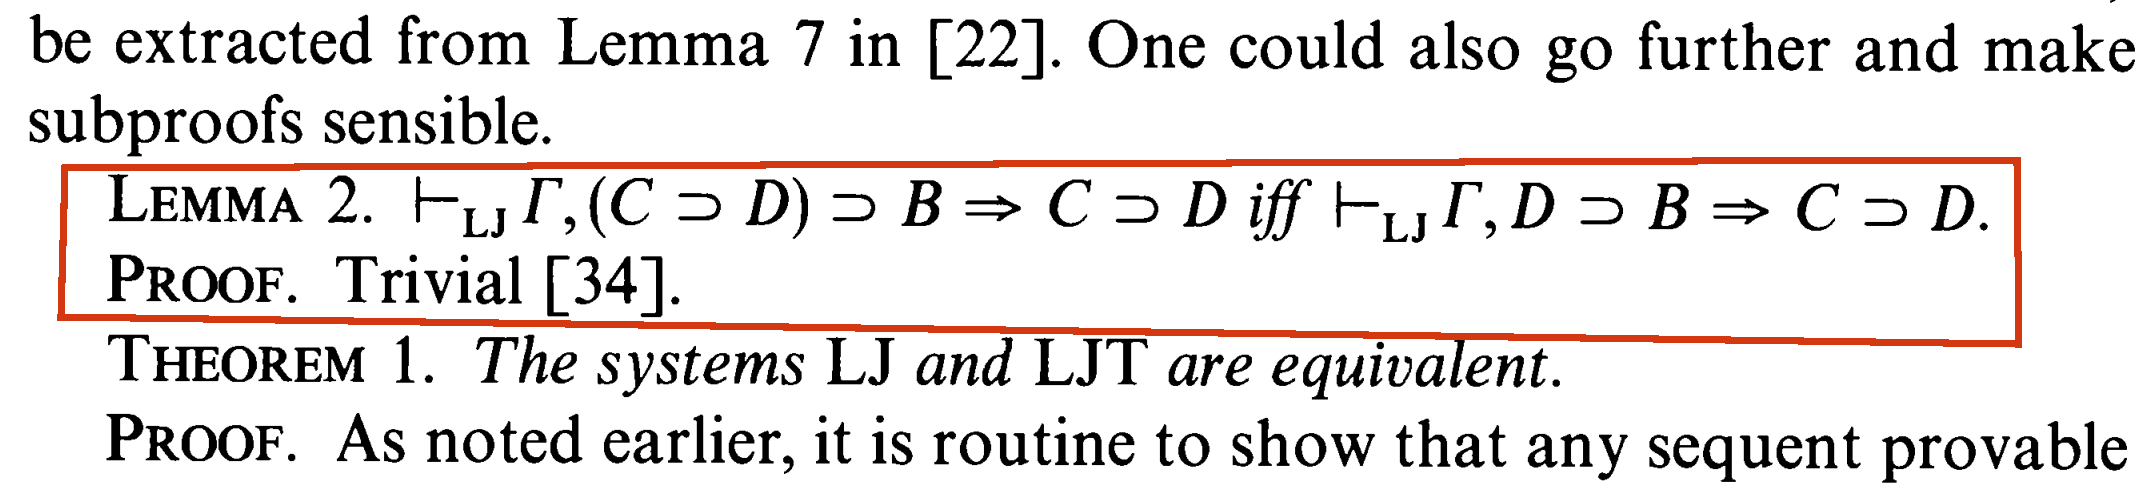
\includegraphics[width=0.8\textwidth]{Vorobieff-lemma}
\par\end{center}

\begin{center}
{\footnotesize{}{[}R. Dyckhoff, }\emph{\footnotesize{}Contraction-Free
Sequent Calculi for Intuitionistic Logic}{\footnotesize{}, 1992{]}}
\par\end{center}{\footnotesize \par}
\begin{itemize}
\item A stepping stone to this theorem:{\footnotesize{}
\[
\left(\left(A\Rightarrow B\right)\Rightarrow C\right)\Rightarrow B\Rightarrow C
\]
}Proof (\emph{obviously} trivial): $f^{\left(A\Rightarrow B\right)\Rightarrow C}\Rightarrow b^{B}\Rightarrow f\:(x^{A}\Rightarrow b)$
\begin{itemize}
\item \emph{Details are left as exercise for the reader}
\end{itemize}
\end{itemize}
\end{frame}

\begin{frame}{Proof search V: From deduction rules to code}

\begin{itemize}
\item The new rules are equivalent to the old rules, therefore...
\begin{itemize}
\item Proof of a sequent $A,B,C\vdash G$ $\Leftrightarrow$ code/expression
$t(a,b,c):G$
\item Also can be seen as a function $t$ from $A,B,C$ to $G$
\end{itemize}
\item Sequent in a proof follows from an axiom or from a transforming rule
\begin{itemize}
\item The two axioms are fixed expressions, $x^{A}\Rightarrow x$ and $1$
\item Each rule has a \emph{proof transformer} function: $\text{PT}_{R\Rightarrow}$
, $\text{PT}_{L+}$ , etc.
\end{itemize}
\item Examples of proof transformer functions:
\begin{align*}
\frac{\Gamma,A\vdash C\quad\;\Gamma,B\vdash C}{\Gamma,{\color{blue}A+B}\vdash C}\:L+\\
PT_{L+}(t_{1}^{A\Rightarrow C},t_{2}^{B\Rightarrow C})=x^{A+B}\Rightarrow & \ x\ \text{match}\begin{cases}
a^{A}\Rightarrow t_{1}(a)\\
b^{B}\Rightarrow t_{2}(b)
\end{cases}
\end{align*}
\begin{align*}
\frac{\Gamma,A\Rightarrow B\Rightarrow C\vdash D}{\Gamma,{\color{blue}(A\times B)\Rightarrow C}\vdash D}\:L\Rightarrow_{2}\\
PT_{L\Rightarrow_{2}}(f^{\left(A\Rightarrow B\Rightarrow C\right)\Rightarrow D})=g^{A\times B\Rightarrow C}\Rightarrow & f\,(x^{A}\Rightarrow y^{B}\Rightarrow g(x,y))
\end{align*}
\item Verify that we can indeed produce PTs for every rule of LJT
\end{itemize}
\end{frame}

\begin{frame}{Proof search example II: deriving code}

Once a proof tree is found, start from leaves and apply PTs
\begin{itemize}
\item For each sequent $S_{i}$, this will derive a \textbf{proof expression}
$t_{i}$
\item Example: to prove $S_{0}$, start from $S_{6}$ backwards:{\footnotesize{}
\begin{align*}
S_{6}:\left(R\Rightarrow R\right)\Rightarrow Q;R\vdash R\quad(\text{axiom }Id)\quad & t_{6}(rrq,r)=r\\
S_{2}:\left(R\Rightarrow R\right)\Rightarrow Q\vdash\left(R\Rightarrow R\right)\quad\text{PT}_{R\Rightarrow}(t_{6})\quad & t_{2}(rrq)=\left(r\Rightarrow t_{6}(rrq,r)\right)\\
S_{3}:Q\vdash Q\quad(\text{axiom }Id)\quad & t_{3}(q)=q\\
S_{1}:\left(R\Rightarrow R\right)\Rightarrow Q\vdash Q\quad\text{PT}_{L\Rightarrow}(t_{2},t_{3})\quad & t_{1}(rrq)=t_{3}(rrq(t_{2}(rrq)))\\
S_{0}:\emptyset\vdash\left(\left(R\Rightarrow R\right)\Rightarrow Q\right)\Rightarrow Q\quad\text{PT}_{R\Rightarrow}(t_{1})\quad & t_{0}=\left(rrq\Rightarrow t_{1}(rrq)\right)
\end{align*}
}{\footnotesize \par}
\item The proof expression for $S_{0}$ is then obtained as
\begin{align*}
t_{0} & =rrq\Rightarrow t_{3}\left(rrq\left(t_{2}\left(rrq\right)\right)\right)=rrq\Rightarrow rrq(r\Rightarrow t_{6}\left(rrq,r\right)\\
 & =rrq\Rightarrow rrq\left(r\Rightarrow r\right)
\end{align*}
Simplified final code having the required type: 
\[
t_{0}:\left(\left(R\Rightarrow R\right)\Rightarrow Q\right)\Rightarrow Q=\left(rrq\Rightarrow rrq\left(r\Rightarrow r\right)\right)
\]
\end{itemize}
\end{frame}

\begin{frame}{Summary}

\begin{itemize}
\item The CH correspondence maps the type system of each programming language
into a certain system of logical propositions 
\item If that logic is decidable, we can automatically produce code from
type signatures
\item Simply-typed Lambda Calculus corresponds to IPL, which is decidable
\item In practice, many types have more than one implementation
\item To make this into a practical tool, need heuristics or algebraic laws
\item Implementations available in Scala and Haskell
\end{itemize}
\end{frame}

\end{document}
